\section{Animation}


\subsection{Sprites}

\begin{figure}[h]
\centering
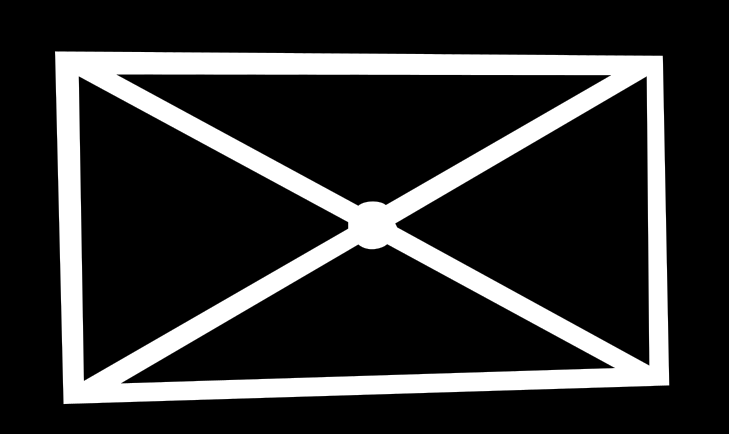
\includegraphics[scale=0.6]{img/mask.png}
\caption{Kleurenmasker van een scherm}
\end{figure}




\subsection{Delaunay}

Voor de animatie wordt gebruik gemaakt van de reeds geschreven delaunay triangulatie. Deze zal het pad vormen waar de kat over zal lopen. Zijn eerste firstPoint en endPoint zijn simpelweg de 2de en 3de punten van de triangulatie (niet 1ste en 2de doordat een rechte lijn als triangle wordt gezien met het eerste punt op de 1ste en 2de positie) \textbf{figuur}. Wanneer de kat zich dicht genoeg bij het endPoint bevindt zal deze de firstPoint worden en zullen de buren van dit punt gezocht worden. Er zal willeukeurig een punt worden gekozen als nieuw endPoint. Er zal ook gekeken worden dat dit punt niet het firstPoint was van de vorige beweging. Dit wil zeggen dat de animatie nooit terug op zijn stappen komt. Enkel als de triangulatie een rechte lijn vormt zal de kat op en neer lopen. Onze kat bestaat uit een sprite file met 8 frames. Deze worden om de beurt getekent om een beweging te simuleren. \textbf{figuur}. Er zal ook gekeken worden naar de orientatie van de lijnen en de richting. Als er van rechts naar links wordt gelopen zal er op het canvas een mirror methode worden toegepast de sprite zal worden getekent en het canvas zal terug gerestored worden. Voor de rotatie zal het canvas naar het centrum van de sprite worden verplaatst, een rotatie zal plaatsvinden waarna weeral een restore van het canvas.\textbf{figuur}

